\chapter{Detalles de Implementación y Experimentos}\label{chapter:implementation}

\section{Detalles de implementaci\'on}

En esta secci\'on se abordar\'an algunos detalles que se tuvieron en cuenta a la hora de implementar este m\'odulo.

\subsection{Modelos}

Primeramente obs\'ervese que el rango de niveles de gris de una imagen se define como $[0,M)$. Por ende al transformar la imagen a una funci\'on de tono de gris utilizando la f\'ormula (1.11) cuando el nivel de gris es 0 el tono de gris es $M$, lo cual contradice que el rango de tono de gris para el modelo LIP es $[0,M)$. Por este motivo tanto para la clase \verb|LIPImage| como \verb|LIPSpace| antes de cambiar la imagen de niveles de gris a tonos de gris y viceversa esta primero se procesa de tal forma que el menor valor admisible sea un n\'umero cercano a cero pero mayor que este. En esta implementaci\'on se decidi\'o utilizar el n\'umero $0.0001$. No se opt\'o por otro alternativas como por ejemplo el \'epsilon de la m\'aquina porque al realizar operaciones aritm\'eticas este valor se convert\'ia en cero y por ende no solucionaba el problema planteado. Esta tambi\'en se hizo en la implementaci\'on del modelo PLIP. Para el caso del modelo SLIP no fue necesario pues se utiliza una funci\'on de tono de gris, se trabaja directamente con los niveles de gris.

Otro problema que fue necesario resolver es que en el modelo HLIP los niveles de gris de la imagen a transformar deben estar en el rango $(0,M)$. La soluci\'on propuesta fue hacer algo similar al caso anterior pero solo antes de cambiar la imagen de nivel de gris a tono de gris.

Las implementaciones de todos los modelos tal y como se explic\'o en el cap\'itulo anterior se puede encontrar en el subm\'odulo ``models'', cada uno en su archivo correspondiente.

\subsection{M\'etricas}

Como se explic\'o en el cap\'itulo exterior se implementaron dos m\'etricas: EMEE y $C_p(p)$. La implementaci\'on de estas m\'etricas se puede encontrar en el subm\'odulo ``metrics''. Este subm\'odulo consta de dos archivos: ``emee.py'' y ``contrast\_pixel''. 

\subsubsection{EMEE}
En el archivo ``emee.py'' se encuentran dos funciones: \verb|emee| y \verb|find_min_max|. La primera devuelve el valor de EMEE de una imagen dada como entrada. Adem\'as recibe como par\'ametros el valor de $\alpha$, las dimensiones de los bloques en los que se desea dividir la imagen y una constante $c$. Esta constante se utiliza para evitar la divisi\'on por $0$ en (1.33). Se suma tanto al numerador como al denominador de las fracciones que aparecen. La constante que se utiliz\'o para calcular los mejores par\'ametros fue $0.5$. Esto tambi\'en para evitar que una divisi\'on por un n\'umero muy cercano a 0 diera un resultado demasiado grande. 

La funci\'on \verb|find_min_max| se utiliza para calcular el menor y mayor valor de intensidad de un bloque. Da como salida una tupla con dicho valores en ese orden y recibe una imagen y 4 enteros: $n_1,n_2,m_1,m_2$, tal que $(n_1,m_1)$ son las coordenadas donde inicia el bloque y; $n_2$ y $m_2$ son la dimensi\'on horizontal y vertical del bloque respectivamente.

\subsubsection{Contraste Promedio}
En el archivo ``contrast\_pixel.py'' se encuentra tres funciones. La primera funci\'on \verb|abs_contrast_2_pixels| se utiliza para calcular el contraste absoluto entre 2 pixeles. Recibe dos tuplas de 3 elementos, tal que cada una representa representa un pixel (las coordenadas y el valor de intensidad del pixel), y el valor de $M$.  La segunda funci\'on \verb|contras_pixel| calcula el contraste de un pixel en una imagen; recibe como par\'ametros una tupla que representa al pixel, la imagen, el valor de $M$ y un valor $v$ que indica el radio de la vecindad a considerarse. 

La \'ultima funci\'on \verb|contrast_img| da como salida el contraste promedio de un pixel en una imagen, o sea $C_p$. Esta funci\'on recibe como par\'ametros la imagen, el valor de $M$ y el radio de la vecindad que se debe tener en cuenta alrededor de un pixel. Como calcular el contraste para cada pixel de una imagen es un proceso que puede demorar seg\'un el tama\~no de la imagen, se tom\'o la decisi\'on de, para imagen cuya resoluci\'on fuese mayor que $300\times300$, escoger un subconjunto de pixeles. El criterio para escoger dichos pixeles fue el siguiente:

\begin{enumerate}
	\item Iniciar desde la posici\'on $(0,0)$
	\item Si se analiz\'o el pixel en la posici\'on $(i,j)$ el pr\'oximo pixel a analizar es el pixel $(i,j+3)$
	\item Una vez terminada de analizar una fila $i$ la pr\'oxima fila a analizar es la fila $i+3$.
\end{enumerate}

El radio de la vecindad que se tom\'o para calcular el contraste de cada pixel fue de 2. Al comparar ambas formas se pudo comprobar que, para im\'agenes con una resoluci\'on grande, la forma propuesta, reduce considerablemente el tiempo de ejecuci\'on, afectando en una cantidad despreciable el resultado final.

\subsection{Algoritmos}

La implementaci\'on de los algoritmos explicados en el cap\'itulo anterior se encuentra en el subm\'odulo ``algorithms''. Este subm\'odulo se compone de tres archivos: ``edge\_detection'', ``unsharp\_masking'' y ``affine\_transform.py''.

\subsubsection{Detecci\'on de Bordes}

El archivo ``edge\_detection'' tiene implementadas dos funciones: \verb|edge_detection| y \verb|space_edge_detection|. La primera recibe como par\'ametros una imagen y un filtro y da como salida el resultado de aplicarle el filtro a la imagen. 

La segunda funci\'on, adem\'as de recibir estos mismos par\'ametros, recibe una instancia de tipo \verb|LogSpace|. Este se utiliza para indicar el modelo que se desea a utilizar. El funcionamiento es sencillo: se transforma la imagen al isomorfismo utilizando primeramente la funci\'on de cambio a tonos de gris y luego la funci\'on del isomorfismo, se aplica el filtro a la imagen transformada y se regresa este resultado al espacio original utilizando primero la inversa de la funci\'on del isomorfismo y luego la funci\'on de cambio a niveles de gris. Recu\'erdese que los modelos que no utilizan funciones de cambio, en su implementaci\'on, dan como salida la misma imagen dada de entrada.

\subsubsection{Unsharp Masking}

El archivo ``unsharp\_masking.py'' consta de dos funciones: \verb|unsharp_masking| y \verb|space_unsharp_masking|. La primera recibe como par\'ametros una imagen, un filtro y un \textit{string} que puede ser: \verb|``+''| o \verb|``-''|. La salida de esta funci\'on es el resultado de utilizar el filtro para detectar los bordes de la imagen y fusionar la imagen original y la imagen de bordes utilizando la suma (\verb|``+''|) o la resta (\verb|``-''|) lineal. 

La segunda funci\'on, adem\'as de recibir estos mismos par\'ametros, recibe una instancia de tipo \verb|LogSpace|. Este algoritmo primero transforma la imagen al isomorfismo utilizando primeramente la funci\'on de cambio a tonos de gris y luego la funci\'on del isomorfismo, se aplica el filtro dado y luego seg\'un el operador especificado, a la imagen original se le suma o se le resta la imagen de bordes. Finalmente se utilizan la inversa del isomorfismo y la imagen de cambio a niveles de gris para regresar al espacio original. El permitir que la que fusi\'on, adem\'as de con la suma se haga con la resta, se tom\'o como decisi\'on despu\'es de que uno de los modelos mostr\'o buenos resultados utilizando la resta en lugar de la suma. 

\subsubsection{Transformaci\'on Af\'in}

El archivo ``affine\_transform.py'' contiene dos funciones: \verb|affine_transform| y \verb|space_affine_transform|. La primera da como salida la transformaci\'on af\'in explicada en el cap\'itulo anterior utilizando las operaciones aritm\'eticas lineales. Recibe como par\'ametros una imagen y los extremos del intervalo en el cual se va a realizar la transformaci\'on. 

La segunda funci\'on da como salida la transformaci\'on af\'in utilizando las operaciones aritm\'eticas de un modelo espec\'ifico. Adem\'as de recibir los mismos par\'ametros que la funci\'on, recibe una instancia de tipo \verb|LogSpace|. Este par\'ametro se utiliza para indicar con que modelo se quiere realizar la transformaci\'on. Los extremos del intervalo de entrada deben ser los del modelo utilizado para obtener los mejores resultados.

\section{Experimentos}
Para los experimentos que a continuaci\'on se muestran se utilizaron im\'agenes en escala de gris de 8 bits, o sea que los valores de intensidades de los pixeles eran n\'umeros enteros en el intervalo $[0,255]$.  

\subsection{Curvas de los isomorfismos}
Lo primero que se muestra son las curvas de los diferentes isomorfismos, iniciando por los no parametrizados que se muestran en la Fig 3.1. Para los isomorfismos LIP y PSLIP se muestra adem\'as los puntos respectivos a los valores: 0 (rojo), 128 (naranja) y 255(amarillo). Para el caso de HLIP se muestran los puntos para los valores: 1 (rojo), 128 (naranja) y 255 (amarillo). Para el caso del modelo SLIP se muestran los puntos para los valores: -255 (morado) -128(verde) 0 (rojo), 128 (naranja) y 255(amarillo).

\begin{figure}
	\begin{center}
		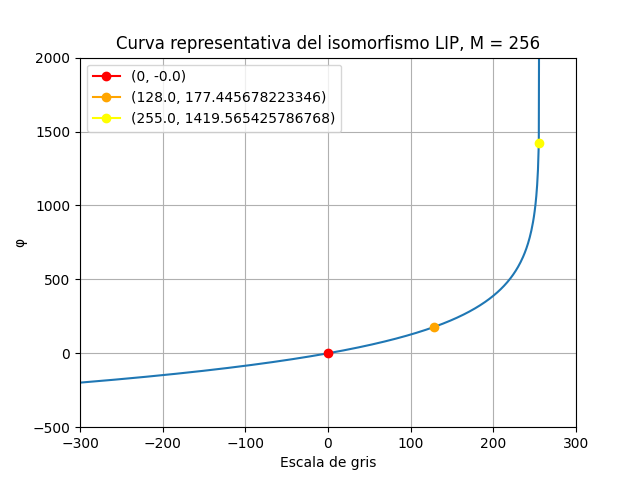
\includegraphics[width=5.5 cm]{images/clasics_curves/lip_curve.png}
		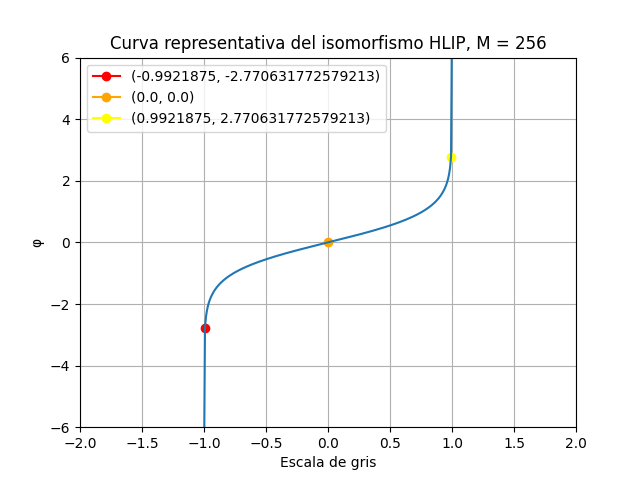
\includegraphics[width=5.5 cm]{images/clasics_curves/hlip_curve.png}
		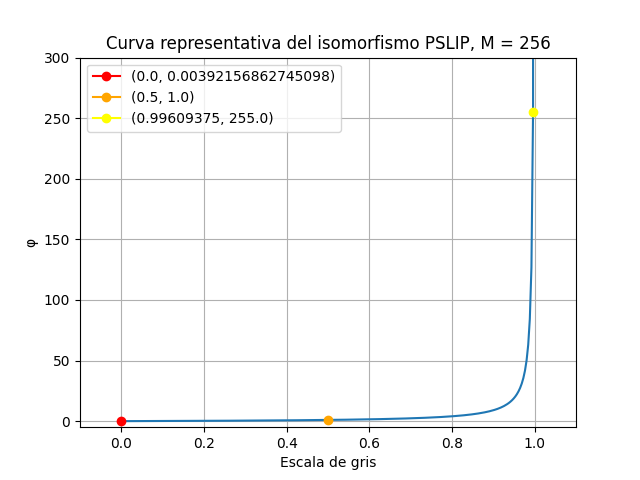
\includegraphics[width=5.5 cm]{images/clasics_curves/pslip_curve.png}
		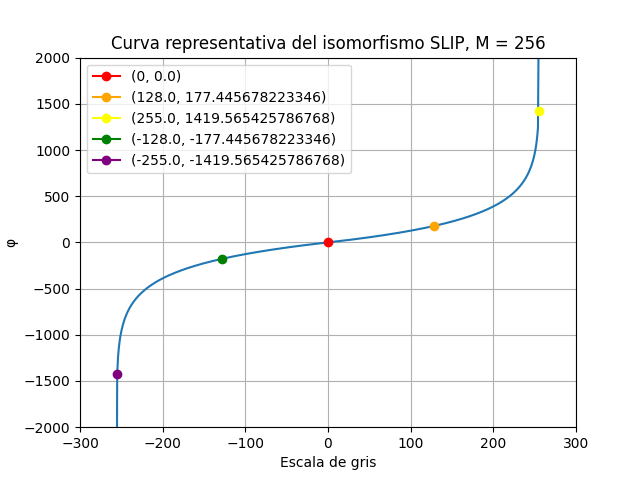
\includegraphics[width=5.5 cm]{images/clasics_curves/slip_curve.png}
		\caption{Curvas representativas de los modelos no parametrizados}
	\end{center}
\end{figure}

En las Fig 3.2 y Fig 3.3 se pueden observar varias curvas del modelo PLIP y PPSLIP utilizando diferentes valores de $\lambda(M)$. En ambos modelos se puede apreciar la tendencia a la linealidad a medida que el valor de $\lambda(M)$ aumenta. Obse\'ervese que los puntos correspondiente a 0 (rojo), 128 (naranja) y 255 (amarillo) se van acercando a una l\'inea recta. Tambi\'en se muestra que los nuevos valores que aparecen siguen manteniendo la estructura logar\'itmica.

\begin{figure}
	\begin{center}
		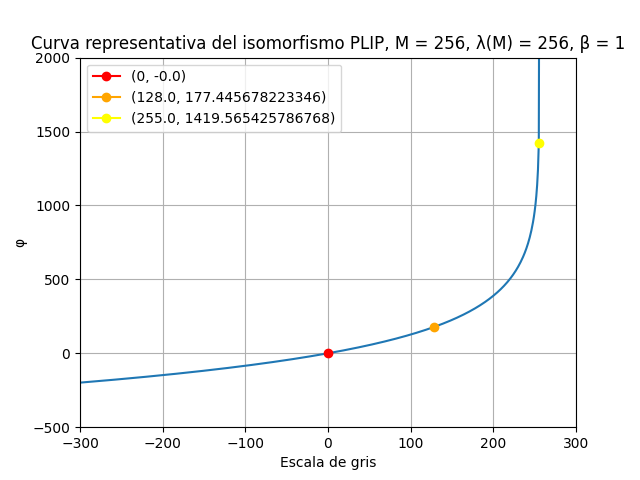
\includegraphics[width=5.5 cm]{images/plip_curves/plip_curve_256.png}
		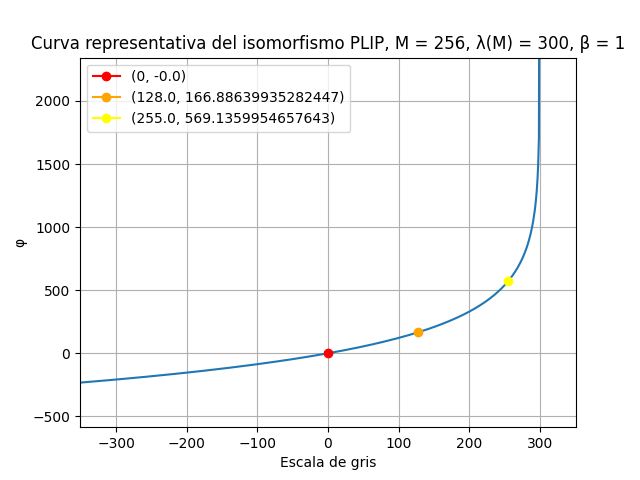
\includegraphics[width=5.5 cm]{images/plip_curves/plip_curve_300.png}
		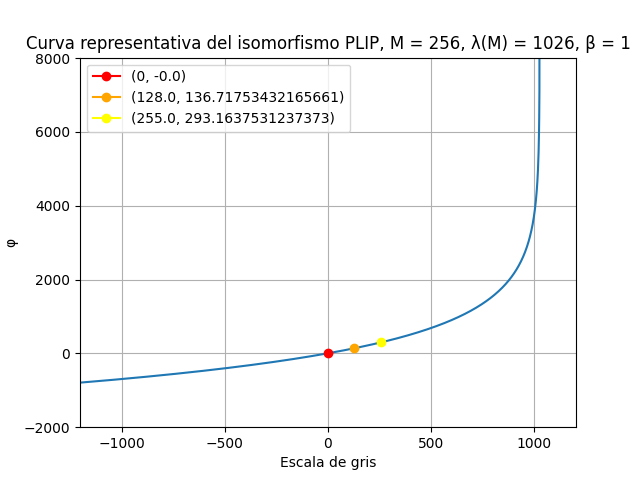
\includegraphics[width=5.5 cm]{images/plip_curves/plip_curve_1026.png}
		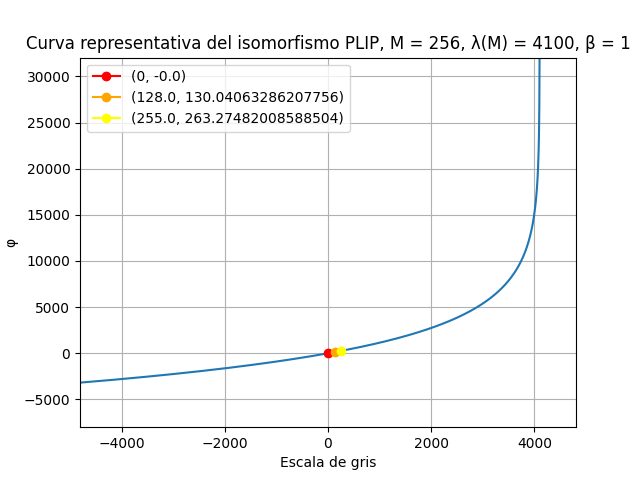
\includegraphics[width=5.5 cm]{images/plip_curves/plip_curve_4100.png}
		\caption{Curvas representativas del modelo PLIP con diferentes valores de $\lambda(M)$}
	\end{center}
\end{figure}

\begin{figure}
	\begin{center}
		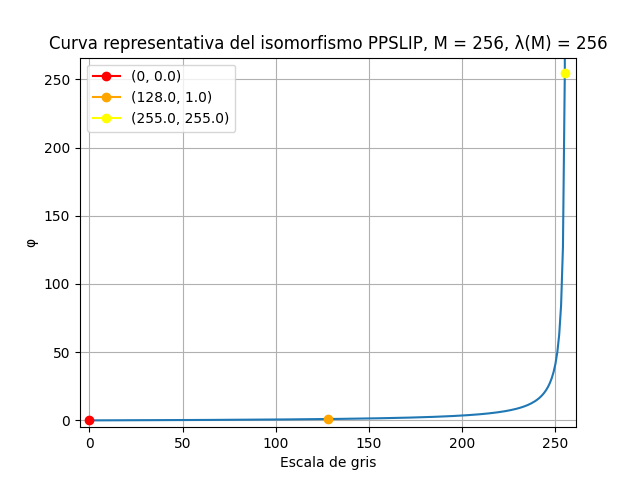
\includegraphics[width=5.5 cm]{images/ppslip_curves/ppslip_curve_256.png}
		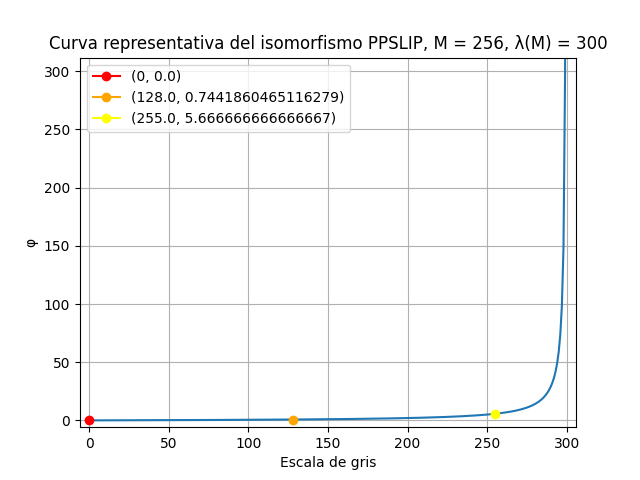
\includegraphics[width=5.5 cm]{images/ppslip_curves/ppslip_curve_300.png}
		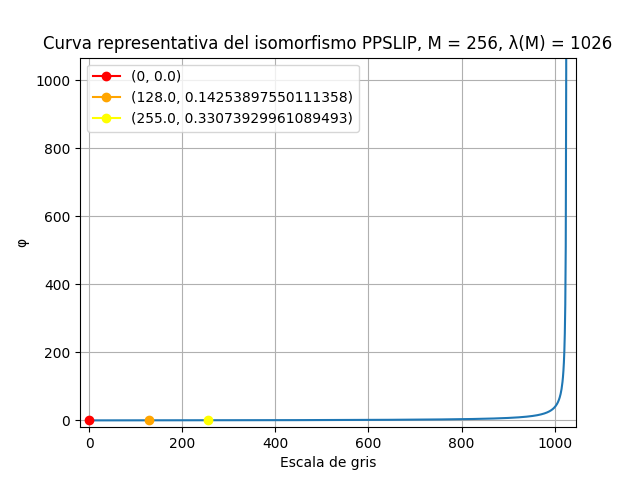
\includegraphics[width=5.5 cm]{images/ppslip_curves/ppslip_curve_1026.png}
		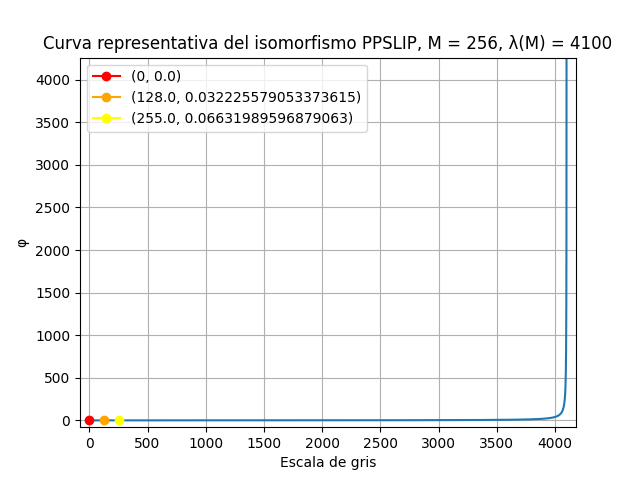
\includegraphics[width=5.5 cm]{images/ppslip_curves/ppslip_curve_4100.png}
		\caption{Curvas representativas del modelo PPSLIP con diferentes valores de $\lambda(M)$}
	\end{center}
\end{figure}

\subsection{Suma de im\'agenes}

Uno de las formas m\'as utilizadas para la fusi\'on de im\'agenes es la suma de las mismas. Para los experimentos que se muestran a continuaci\'on se utilizar\'an las im\'agenes: Motorista, Esqu\'i, Patineta y Playa que se muestran en la Fig 3.4.

\begin{figure}
	\begin{center}
		\subfigure[Motorista]{
		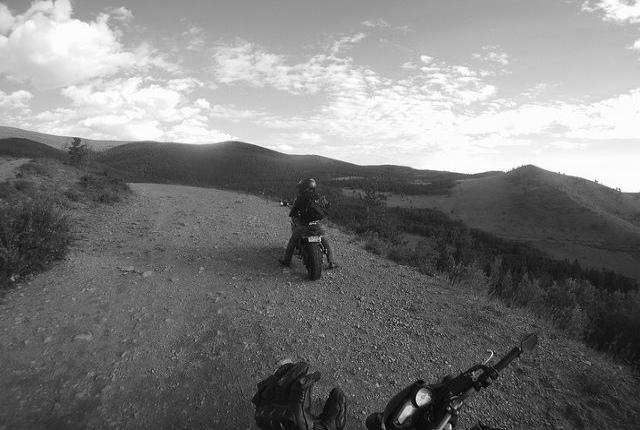
\includegraphics[width=5.5 cm]{images/originals/motorista.jpg}}
		\subfigure[Esqu\'i]{
			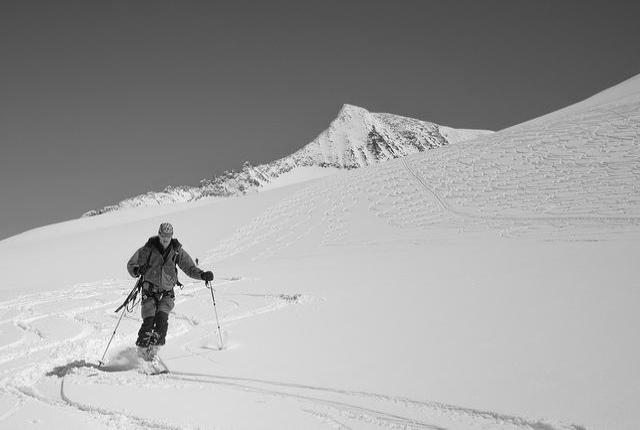
\includegraphics[width=5.5 cm]{images/originals/esqui.jpg}}
		\subfigure[Patineta]{
			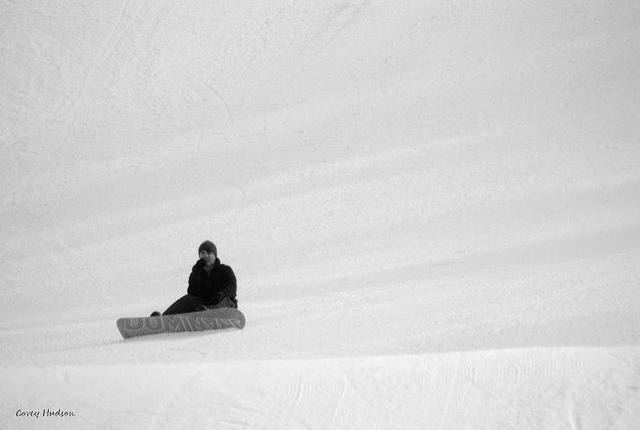
\includegraphics[width=5.5 cm]{images/originals/patineta.jpg}}
		\subfigure[Playa]{
			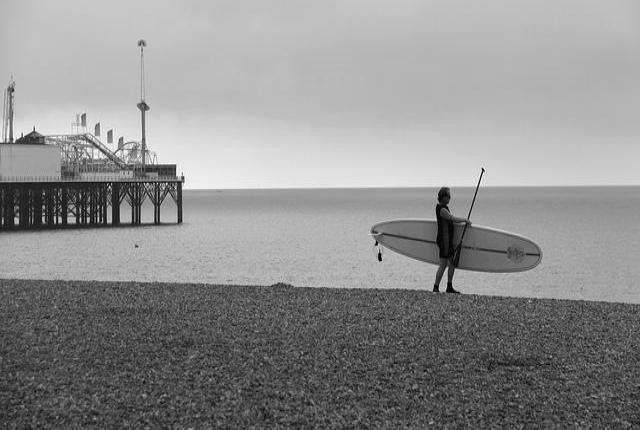
\includegraphics[width=5.5 cm]{images/originals/playa.jpg}}
		\caption{Im\'agenes para los experimentos de suma}
	\end{center}
\end{figure}

\begin{figure}
	\begin{center}
		\subfigure[Lineal $C_p=63.93$]{
			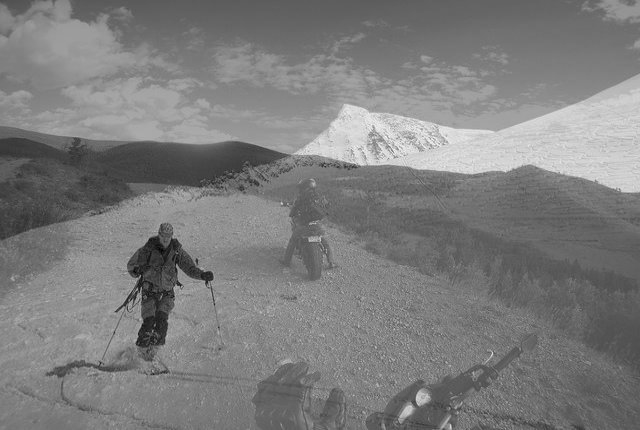
\includegraphics[width=5.5 cm]{images/sums/m y e/sab.png}}
		\subfigure[LIP $C_p=62.97$]{
			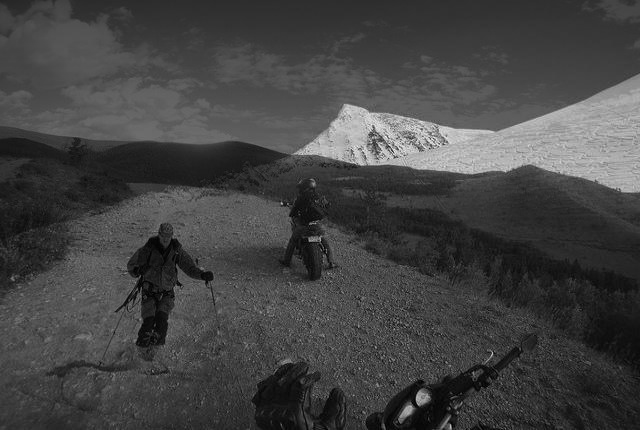
\includegraphics[width=5.5 cm]{images/sums/m y e/jsab.png}}
		\subfigure[HLIP $C_p=66.25$]{
			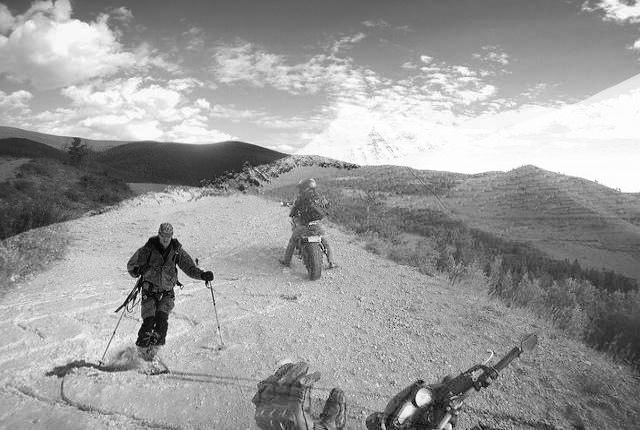
\includegraphics[width=5.5 cm]{images/sums/m y e/hsab.png}}
		\subfigure[PSLIP $C_p=59.91$]{
			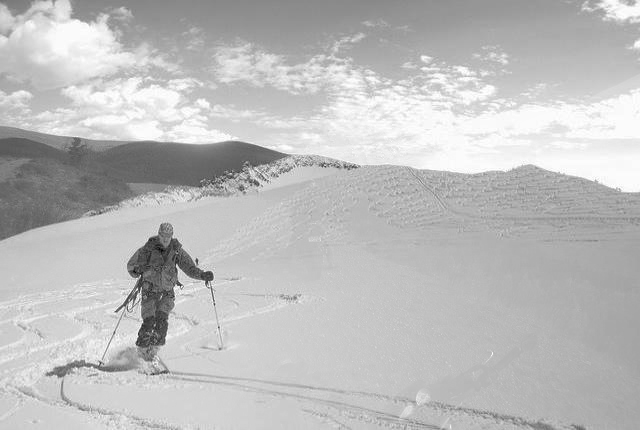
\includegraphics[width=5.5 cm]{images/sums/m y e/pssab.png}}
		\subfigure[SLIP $C_p=62.71$]{
			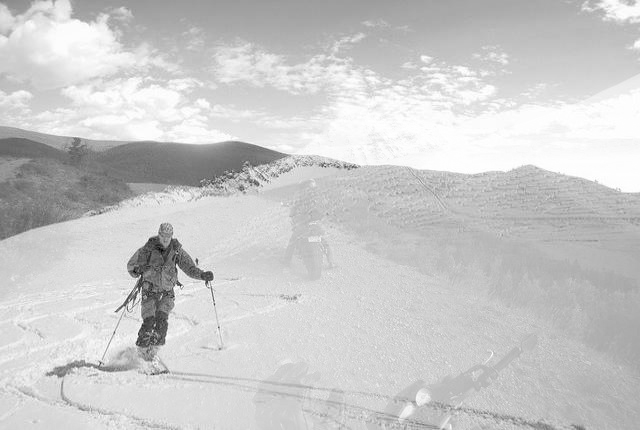
\includegraphics[width=5.5 cm]{images/sums/m y e/ssab.png}}
		\subfigure[PLIP $C_p=63.98$]{
			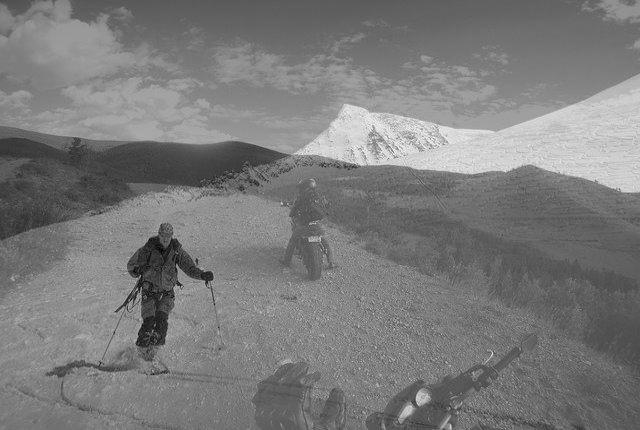
\includegraphics[width=5.5 cm]{images/sums/m y e/psab.png}}
		\subfigure[PPSLIP $C_p=63.87$]{
			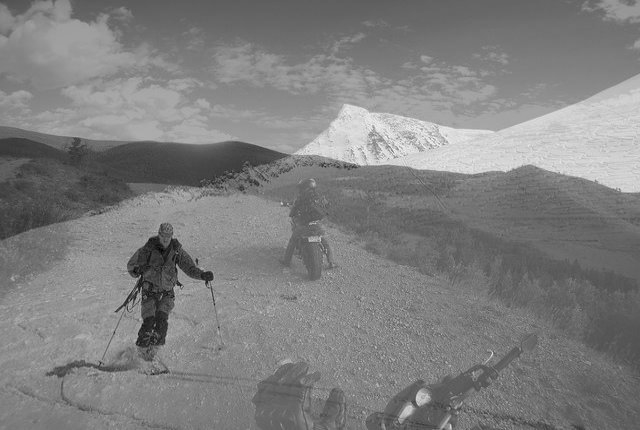
\includegraphics[width=5.5 cm]{images/sums/m y e/ppssab.png}}
		\caption{Suma de Motorista y Esqu\'i utilizando los diferentes modelos}
	\end{center}
\end{figure}

\begin{figure}
	\begin{center}
		\subfigure[Lineal $C_p=62.27$]{
			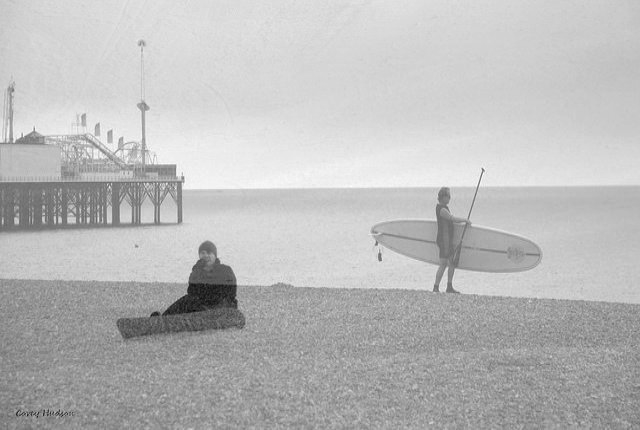
\includegraphics[width=5.5 cm]{images/sums/p y p/scd.png}}
		\subfigure[LIP $C_p=66.08$]{
			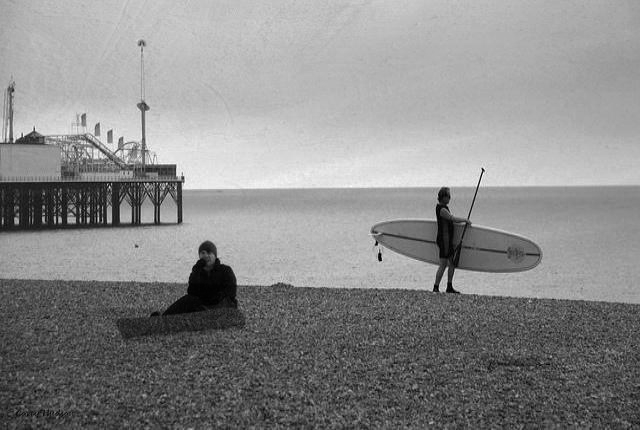
\includegraphics[width=5.5 cm]{images/sums/p y p/jscd.png}}
		\subfigure[HLIP $C_p=59.88$]{
			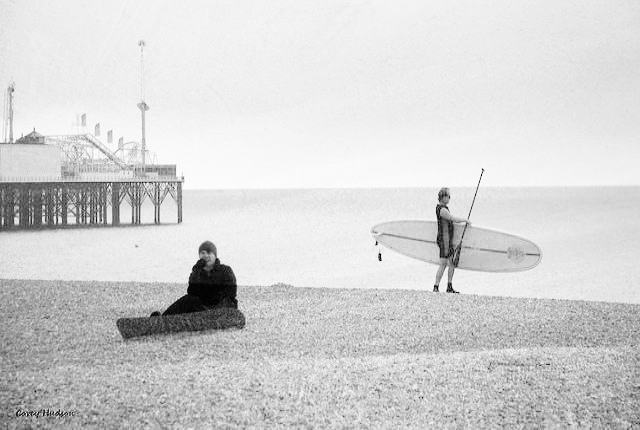
\includegraphics[width=5.5 cm]{images/sums/p y p/hscd.png}}
		\subfigure[PSLIP $C_p=56.85$]{
			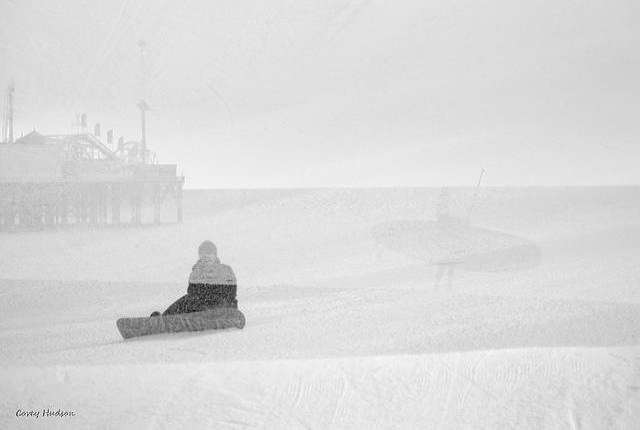
\includegraphics[width=5.5 cm]{images/sums/p y p/psscd.png}}
		\subfigure[SLIP $C_p=52.83$]{
			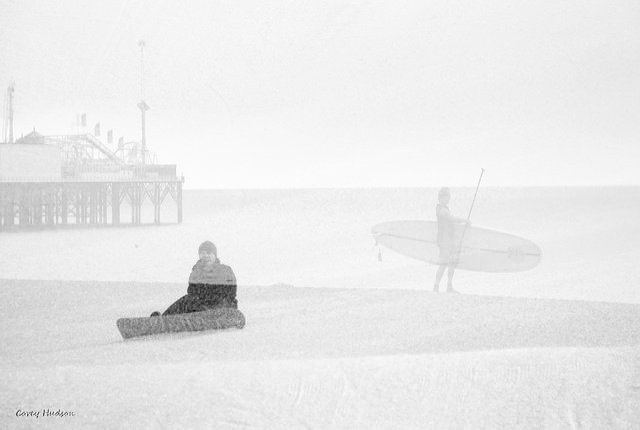
\includegraphics[width=5.5 cm]{images/sums/p y p/sscd.png}}
		\subfigure[PLIP $C_p=66.08$]{
			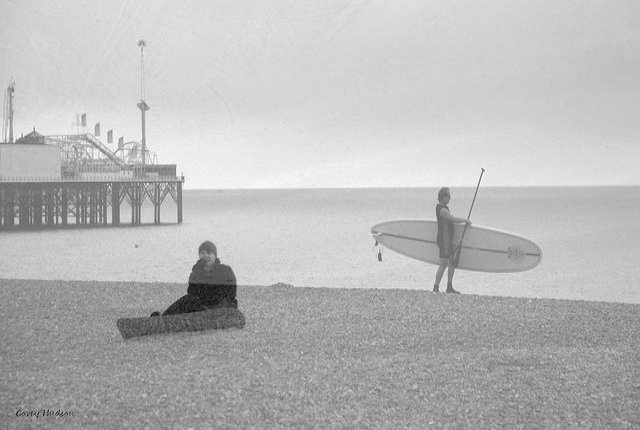
\includegraphics[width=5.5 cm]{images/sums/p y p/pscd.png}}
		\subfigure[PPSLIP $C_p=62.04$]{
			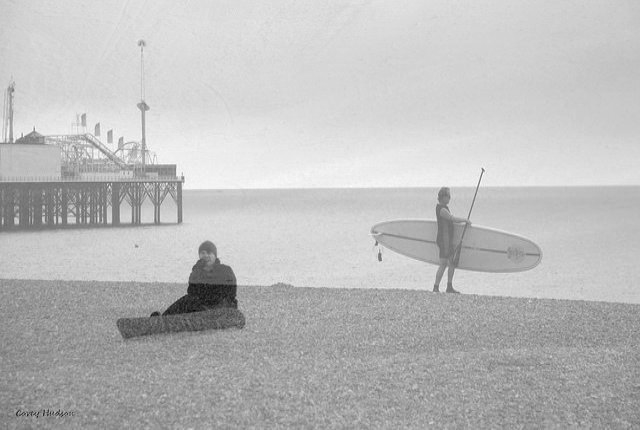
\includegraphics[width=5.5 cm]{images/sums/p y p/ppsscd.png}}
		\caption{Suma de Patineta y Playa utilizando los diferentes modelos}
	\end{center}
\end{figure}

En la figura 3.5 se muestran la suma de la imagen ``Motorista'' y la imagen ``Esqu\'i''. Se puede apreciar como el mejor contraste promedio $C_p$ se tiene en este caso para el modelo HLIP. La imagen para el modelo LIP como es natural es oscura, mientras que para el modelo SLIP es muy clara, esto es obvio pues en el modelo LIP se invierte la escala de grises mientras que en el SLIP no. Tambi\'en se puede apreciar que el modelo PSLIP tiene el peor contraste promedio, adem\'as de que elimin\'o gran parte del contenido de las im\'agenes, por lo que no lo hace muy efectivo en la suma de im\'agenes y como con el modelo parametrizado PPSLIP propuesto se obtiene una mejor imagen. En este caso el modelo PLIP obtuvo un mejor valor de contraste al acercarse a la linealidad.

Para determinar los par\'ametros de $\gamma(M)$ y $\mu(M)$ en el modelo PLIP, se aplic\'o el cambio a tonos de gris utilizando el valor de $M=256$. Luego se prob\'o la suma con diferentes valores de $\gamma(M)$ (256, 300, 1026 y 4100) y por cada uno se probaron varios valores de $\mu(M)$ para cambiar a niveles de grises. Para determinar el mejor valor de $\mu(M)$ para cada $\gamma(M)$ se utiliz\'o la m\'etrica EMEE. Luego se calcul\'o el valor de $C_p$ por cada pareja y se el mejor valor s e obtuvo para $\mu(M)=500$ y $\gamma(M)=4100$. Para determinar el mejor valor de $\gamma(M)$ para el modelo PPSLIP se realiz\'o la operaci\'on de suma utilizando varios par\'ametros y se determin\'o el mejor utilizando la EMEE, el resultado fue de $\gamma(M)=4100$. 

En la figura 3.6 se puede observar otro ejemplo de la suma. En este caso el mejor valor de contraste promedio lo da el modelo LIP y por ende el modelo PLIP tambi\'en arroja este resultado. Se comprueba una vez m\'as que el modelo SLIP y PSLIP no dan buenos resultados con la suma y que el modelo PPSLIP mejora la calidad de la suma. Aqu\'i tambi\'en el valor de $\gamma(M)$ resultante fue 4100.

\subsection{Detecci\'on de Bordes}

En esta secci\'on se muestra una comparaci\'on entre los diferentes modelos utilizando el filtro de Scharr para la detecci\'on de bordes. Para la realizaci\'on de estos experimentos se pueden utilzar las funciones descritas en la secci\'on Detalles de Implementaci\'on o se puede hacer el proceso descrito manualmente. En estos experimentos se utilizaron las im\'agenes: C\'amara y T\'orax que se muestran en la Fig 3.7. La primera es una imagen natural y la segunda una imagen m\'edica de Rayos X. Los experimentos realizados se pueden ver en la Fig 3.8 y Fig 3.9 respectivamente.

\begin{figure}
	\begin{center}
		\subfigure[C\'amara]{
			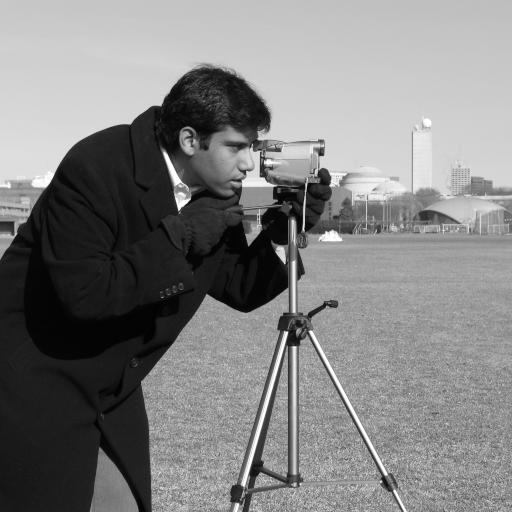
\includegraphics[width=5.0 cm]{images/originals/camera.jpg}}
		\subfigure[T\'orax]{
			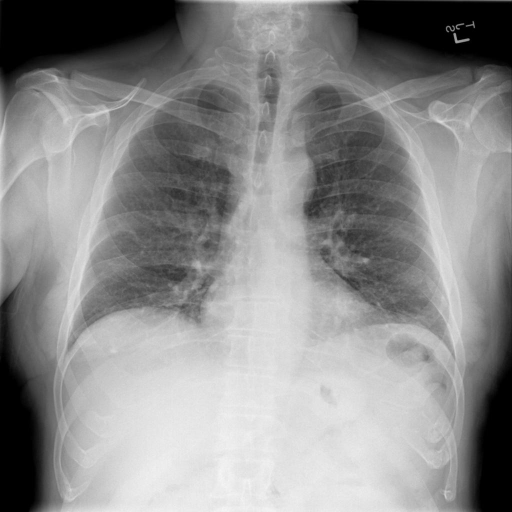
\includegraphics[width=5.0 cm]{images/originals/torax.png}}
		\caption{Im\'agenes para los experimentos de detecci\'on de bordes}
	\end{center}
\end{figure}

\begin{figure}
	\begin{center}
		\subfigure[Lineal $C_p=57.71$]{
			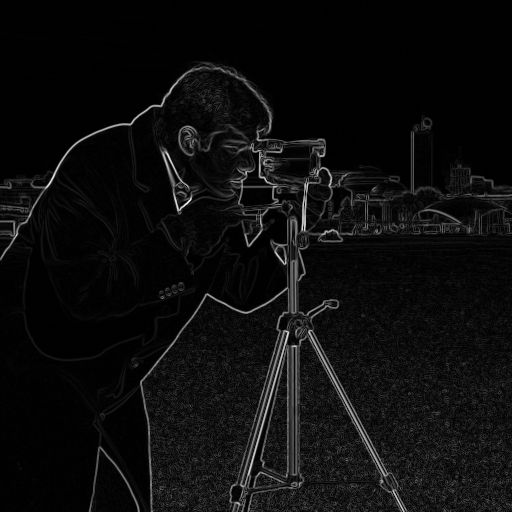
\includegraphics[width=4.0 cm]{images/scharr/camera/sla.png}}
		\subfigure[LIP $C_p=61.45$]{
			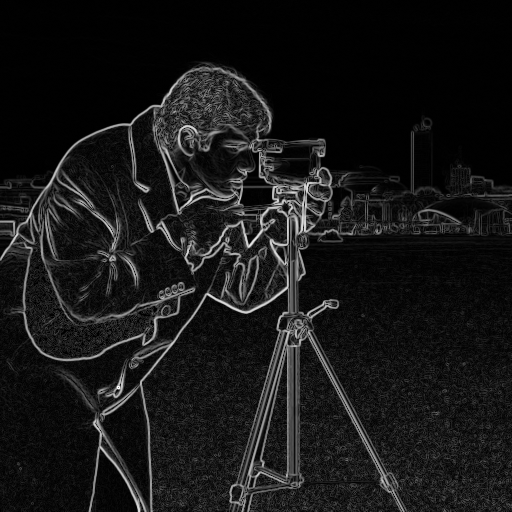
\includegraphics[width=4.0 cm]{images/scharr/camera/sja.png}}
		\subfigure[HLIP $C_p=65.43$]{
			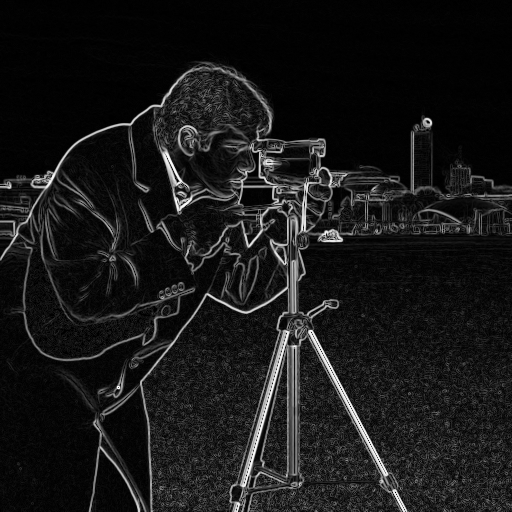
\includegraphics[width=4.0 cm]{images/scharr/camera/sha.png}}
		\subfigure[PSLIP $C_p=66.29$]{
			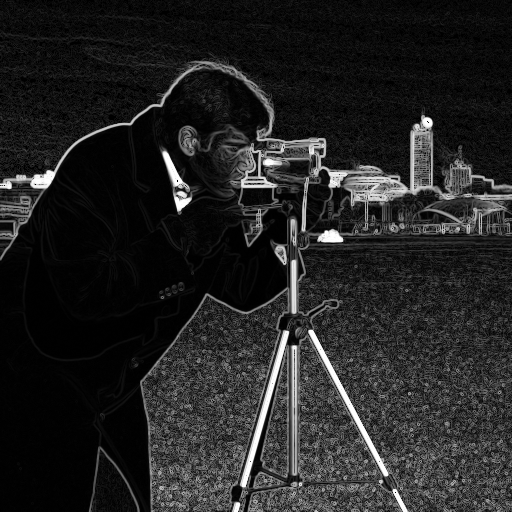
\includegraphics[width=4.0 cm]{images/scharr/camera/spsa.png}}
		\subfigure[SLIP $C_p=63.30$]{
			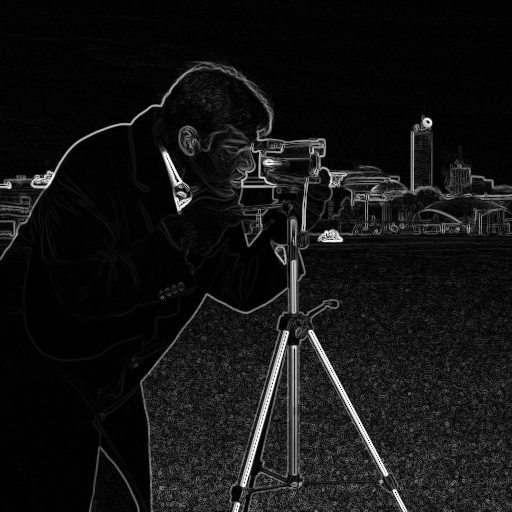
\includegraphics[width=4.0 cm]{images/scharr/camera/ssa.png}}
		\subfigure[PLIP $C_p=61.45$]{
			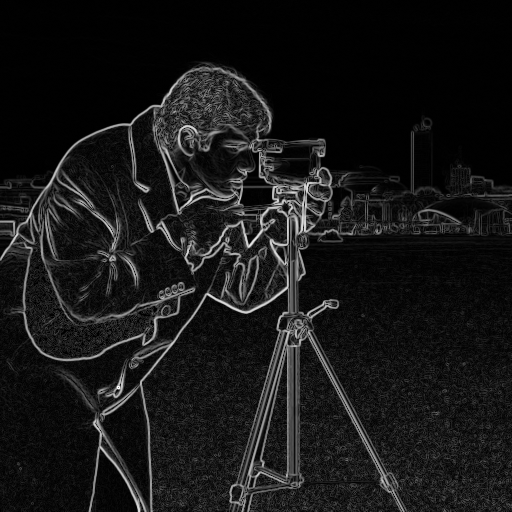
\includegraphics[width=4.0 cm]{images/scharr/camera/spa.png}}
		\subfigure[PPSLIP $C_p=66.29$]{
			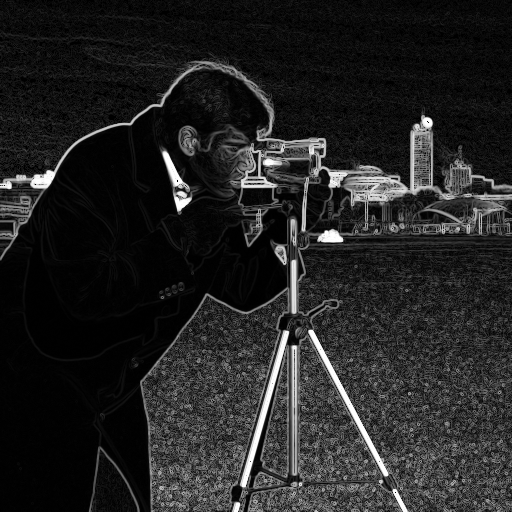
\includegraphics[width=4.0 cm]{images/scharr/camera/sppsa.png}}
		\caption{Filtro de Scharr aplicado a la imagen C\'amara con los diferentes modelos}
	\end{center}
\end{figure}

\begin{figure}
	\begin{center}
		\subfigure[Lineal $C_p=61.85$]{
			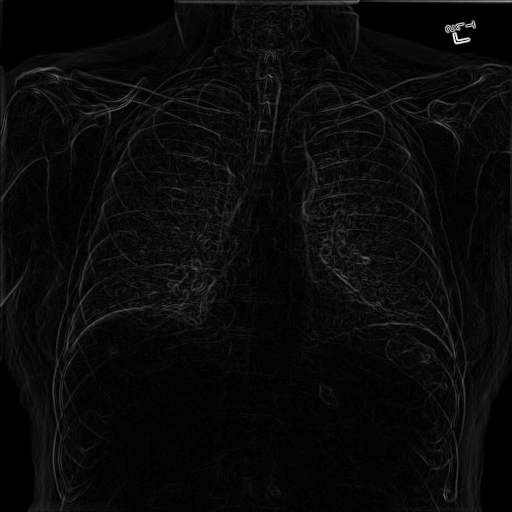
\includegraphics[width=4.0 cm]{images/scharr/torax/slb.png}}
		\subfigure[LIP $C_p=59.01$]{
			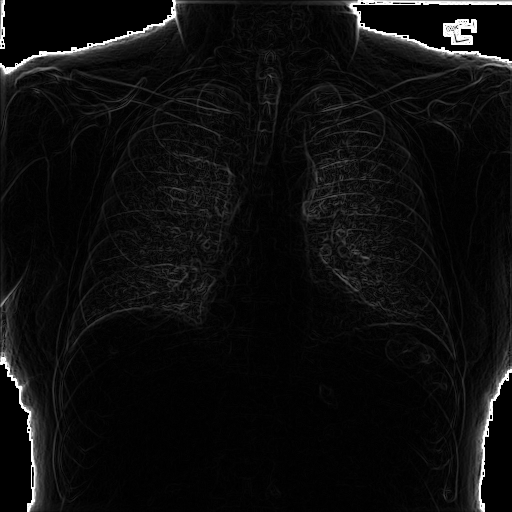
\includegraphics[width=4.0 cm]{images/scharr/torax/sjb.png}}
		\subfigure[HLIP $C_p=63.20$]{
			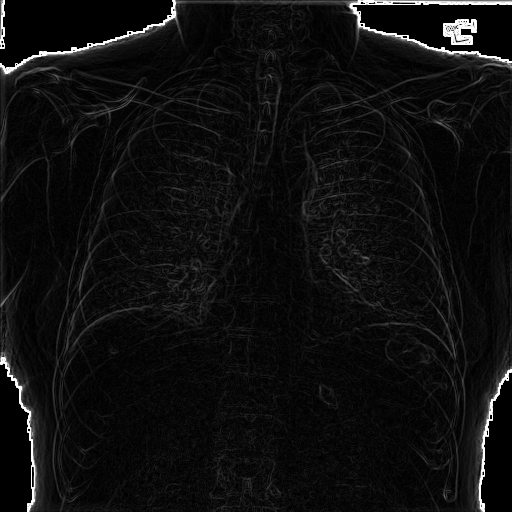
\includegraphics[width=4.0 cm]{images/scharr/torax/shb.png}}
		\subfigure[PSLIP $C_p=65.60$]{
			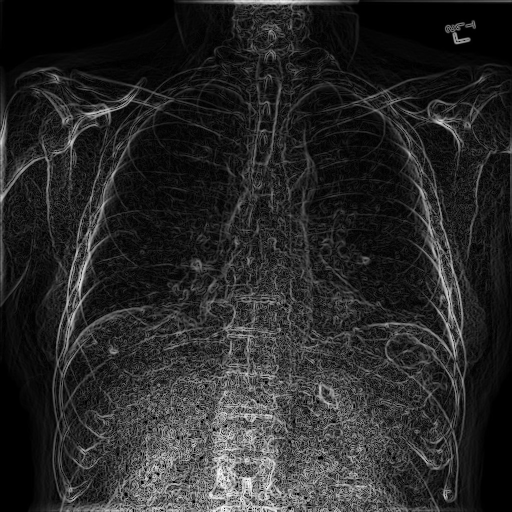
\includegraphics[width=4.0 cm]{images/scharr/torax/spsb.png}}
		\subfigure[SLIP $C_p=65.58$]{
			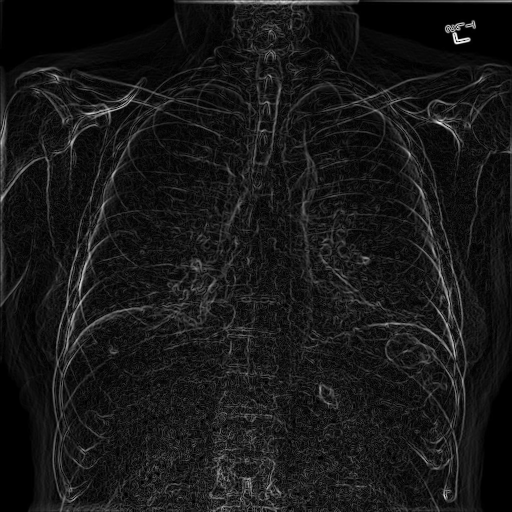
\includegraphics[width=4.0 cm]{images/scharr/torax/ssb.png}}
		\subfigure[PLIP $C_p=61.81$]{
			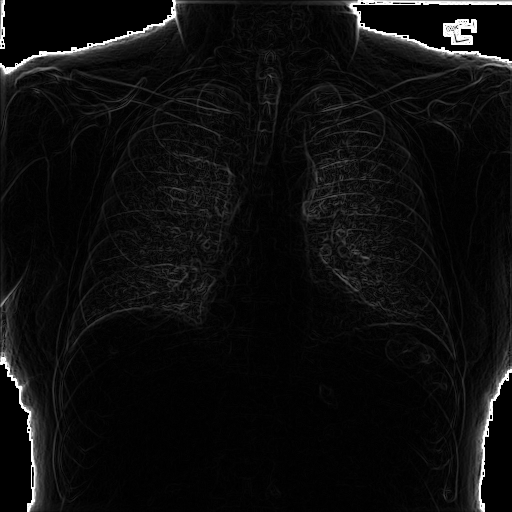
\includegraphics[width=4.0 cm]{images/scharr/torax/spb.png}}
		\subfigure[PPSLIP $C_p=65.60$]{
			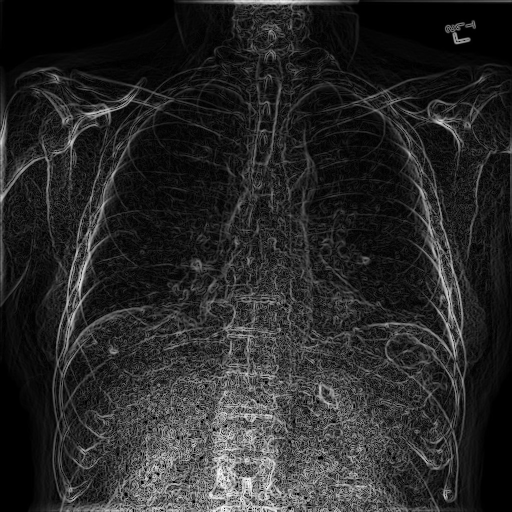
\includegraphics[width=4.0 cm]{images/scharr/torax/sppsb.png}}
		\caption{Filtro de Scharr aplicado a la imagen T\'orax con los diferentes modelos}
	\end{center}
\end{figure} 

Como se puede ver en la Fig 3.8 el modelo lineal se queda bastante rezagado con respecto a los modelos logar\'itmicos en cuanto al contraste promedio $C_p$. Esto adem\'as lo evidencia que el modelo PLIP arroj\'o un resultado similar al modelo LIP. Otro detalle es que el modelo LIP detect\'o mejores los bordes en las tonalidades m\'as oscuras, mientras que el SLIP hizo lo propio para las tonalidades m\'as claras. Clara evidencia esto de a que niveles de gris son m\'as sensibles estos dos modelos. El modelo SLIP por su parte dio un resultado m\'as balanceado arrojando un valor de $C_p$ superior a los anteriores. Sin dudas el mejor resultado se obtuvo utilizando el modelo PSLIP, lo cual se puede comprobar visualmente y mediante el valor de $C_p$, esto gracias a la gran sensibilidad de este modelo a las tonalidades m\'as claras, lo cual era de esperarse al ver la curva de dicho isomorfismo. Dada que este fue el mejor resultado, por ende el modelo PPSLIP coincide con este. Aunque el PSLIP da muy buenos resultados se puede apreciar que para las tonalidades oscuras es superado por el PLIP y el SLIP, una soluci\'on a esto pudiera ser invertir la escala de grises tal como se hace en el modelo LIP, aunque se perder\'ia la gran sensibilidad a tonalidades blancas. Adem\'as se debe tener cuidado ya que su alta sensibilidad lo hace tambi\'en muy sensible al ruido.

En este experimento los par\'ametros a estimar fueron $\lambda(M)$ para PLIP y PPSLIP, adem\'as de $\mu(M)$ en el caso de PPSLIP. La selecci\'on de estos par\'ametros se hizo de una forma similar a la explicada para la suma, lo que obviamente aplicada a la funci\'on del isomorfismo.

Un uso muy pr\'actico es los modelos es la detecci\'on de bordes en im\'agenes m\'edicas. Como se dijo anteriormente un ejemplo de estos se puede apreciar en la Fig 3.9. Dada que es una imagen donde predominan las tonalidades blancas el modelo LIP es el que arroja peores resultados, por ello el modelo PLIP tiende a la linealidad. El modelo HLIP sigue mostrando un comportamiento balanceado y los mejores resultados se obtienen para el modelo PSLIP (y por ende el PPSLIP) y el modelo SLIP.

\subsection{Unsharp Masking}

Los pr\'oximos experimentos que se presentan a continuaci\'on es la aplicaci\'on del algoritmo de \textit{Unsharp Masking} utilizando los diferentes modelos, para la realizaci\'on de los mismos, al igual que en los casos anteriores, se pueden utiliza las funciones implementadas para este cometido y que fueron descritas en la secci\'on ``Detalles de implementaci\'on''. Las im\'agenes utilizadas en estos experimentos ser\'an las mismas ya utilizadas anteriormente: C\'amara y T\'orax. Los resultados de estos experimentos se pueden apreciar en las Fig 3.10 y y 3.11 respectivamente.

\begin{figure}
	\begin{center}
		\subfigure[Original $C_p=58.26$]{
			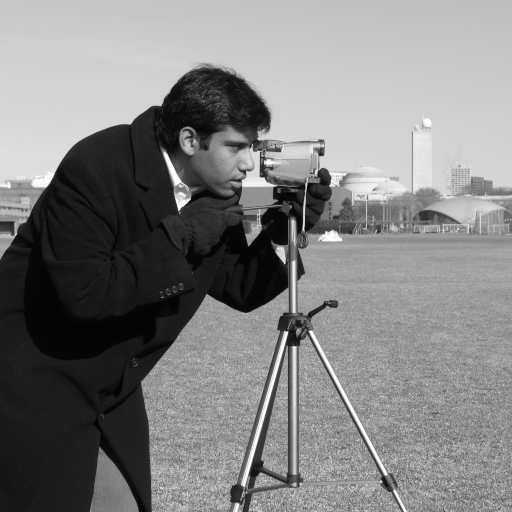
\includegraphics[width=4.0 cm]{images/unsharp_masking/camera/camera.png}}
		\subfigure[Lineal $C_p=56.80$]{
			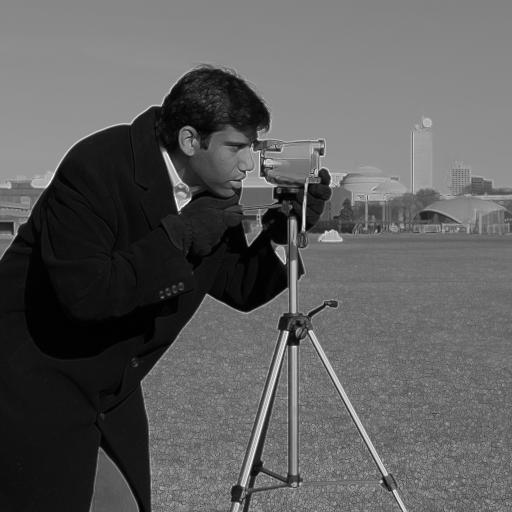
\includegraphics[width=4.0 cm]{images/unsharp_masking/camera/la_sla.png}}
		\subfigure[LIP $C_p=61.21$]{
			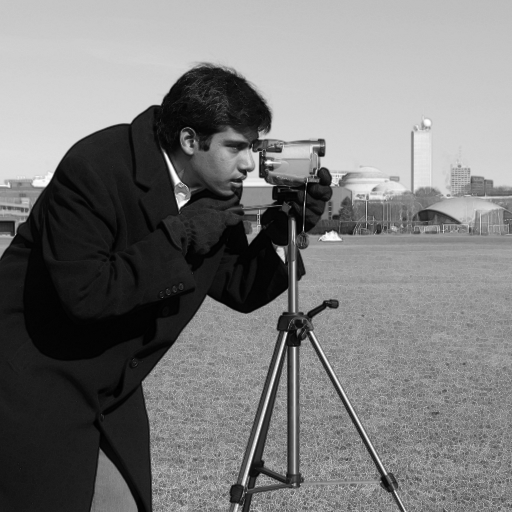
\includegraphics[width=4.0 cm]{images/unsharp_masking/camera/ja_sja.png}}
		\subfigure[HLIP+ $C_p=61.67$]{
			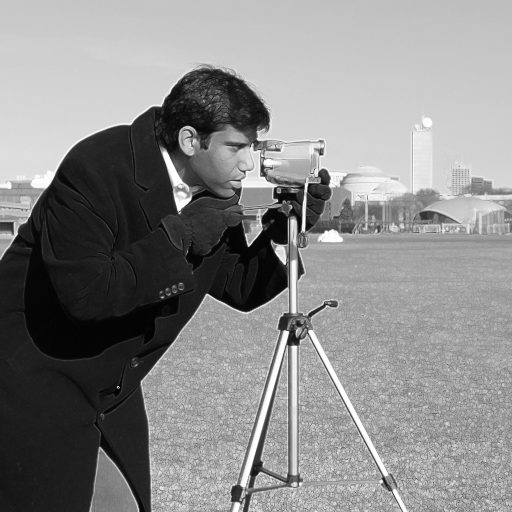
\includegraphics[width=4.0 cm]{images/unsharp_masking/camera/ha_sha+.png}}
		\subfigure[HLIP- $C_p=61.35$]{
			\includegraphics[width=4.0 cm]{images/unsharp_masking/camera/ha_sha-.png}}
		\subfigure[PSLIP $C_p=61.30$]{
			\includegraphics[width=4.0 cm]{images/unsharp_masking/camera/psa_spsa.png}}
		\subfigure[SLIP $C_p=60.63$]{
			\includegraphics[width=4.0 cm]{images/unsharp_masking/camera/sa_ssa.png}}
		\subfigure[PLIP $C_p=61.21$]{
			\includegraphics[width=4.0 cm]{images/unsharp_masking/camera/pa_spa.png}}
		\subfigure[PPSLIP $C_p=65.14$]{
			\includegraphics[width=4.0 cm]{images/unsharp_masking/camera/ppsa_sppsa.png}}
		\caption{Unsharp masking aplicado a la imagen C\'amara con los diferentes modelos}
	\end{center}
\end{figure}

\begin{figure}
	\begin{center}
		\subfigure[Original $C_p=59.91$]{
			\includegraphics[width=4.0 cm]{images/unsharp_masking/torax/CXR7_IM-2263-1001.png}}
		\subfigure[Lineal $C_p=60.99$]{
			\includegraphics[width=4.0 cm]{images/unsharp_masking/torax/lb_slb.png}}
		\subfigure[LIP $C_p=60.70$]{
			\includegraphics[width=4.0 cm]{images/unsharp_masking/torax/jb_sjb.png}}
		\subfigure[HLIP+ $C_p=60.59$]{
			\includegraphics[width=4.0 cm]{images/unsharp_masking/torax/hb_shb+.png}}
		\subfigure[HLIP- $C_p=60.82$]{
			\includegraphics[width=4.0 cm]{images/unsharp_masking/torax/hb_shb-.png}}
		\subfigure[PSLIP $C_p=60.82$]{
			\includegraphics[width=4.0 cm]{images/unsharp_masking/torax/psb_spsb.png}}
		\subfigure[SLIP $C_p=60.99$]{
			\includegraphics[width=4.0 cm]{images/unsharp_masking/torax/sb_ssb.png}}
		\subfigure[PLIP $C_p=60.73$]{
			\includegraphics[width=4.0 cm]{images/unsharp_masking/torax/pb_spb.png}}
		\subfigure[PPSLIP $C_p=63.98$]{
			\includegraphics[width=4.0 cm]{images/unsharp_masking/torax/ppsb_sppsb.png}}
		\caption{Unsharp masking aplicado a la imagen T\'orax con los diferentes modelos}
	\end{center}
\end{figure}

En la Fig 3.11 se puede apreciar como este algoritmo para el caso lineal de una imagen incluso peor a la imagen original pues esta es muy oscura y los bordes no se aprecian muy bien definidos, lo cual tambi\'en los confirma el valor de $C_p$. El modelo LIP da una mejor soluci\'on. Aprovech\'andose el car\'acter sim\'etrico del modelo HLIP se analizaron dos variantes de fusi\'on: la suma y la resta. Si bien el valor de $C_p$ favorece a la fusi\'on con suma, no es mucha la diferencia y visualmente se puede comprobar que la fusi\'on con resta da una imagen de muy buena calidad, la cual podr\'ia considerarse hasta mejor que la arrojada por el algoritmo con la suma. En este sentido es bueno recalcar que $C_p$ es solo una m\'etrica que ha demostrado dar buenos resultados pero no es la \'unica para evaluar la calidad de una imagen y que al final lo m\'as importante es la calidad que percibe un ser humano.

El modelo PSLIP aunque mejora el valor de $C_p$ no es el \'optimo debido a sus problemas con la suma como se vi\'o en el primer experimento. Misma situaci\'on para el SLIP. El modelo PLIP se asemej\'o a un comportamiento logar\'itmico como era de esperarse dados los resultados del modelo lineal y PLIP. Tambi\'en se puede apreciar como el modelo PPSLIP resuelve el problema del modelo PSLIP, arrojando una imagen de mayor calidad, siendo esta la de mejor valor de $C_p$. V\'alido se\~nalar que esta \'ultima resalta mucho los bordes por lo que quiz\'as ser\'ia mejor utilizar otro modelo seg\'un la situaci\'on o utilizar par\'ametros que den una imagen m\'as suave.

Aqu\'i tambi\'en es bueno aclarar que para los modelos parametrizados se utiliz\'o como par\'ametro para la funci\'on del isomorfismo el que di\'o el mejor resultado en la detecci\'on de bordes para cada modelo. Entonces lo que se hizo fue buscar los mejores par\'ametros que dieran el mejor resultado para la fusi\'on.

En la Fig 3.11 si bien todos los modelos resaltan en alguna medida los bordes y mejoran el valor de contraste promedio con respecto a la imagen original, el mejor resultado se logra con el modelo PPSLIP, obteni\'endose una imagen mucho m\'as detallada y de mejor calidad que el resto. Esto confirma una vez m\'as la efectividad y utilidad del modelo propuesto.

\subsection{Transformaci\'on af\'in}

